\subsubsection{压缩映射}
\label{sec:analysis-complete-contraction}

\paragraph{不动点}

对递推$x^{(n+1)}=T(x^{(n)})$，若极限为$x^\star$且可以在更新关系中取极限，
就应有$x^\star=T(x^\star)$。这把寻找一个方程的解与构造收敛序列联系起来。
\begin{definition}[不动点]
\label{def:analysis-fixed-point}
设$T:X\to X$为映射。点$x^\star\in X$若满足$T(x^\star)=x^\star$，就称为$T$的不动点（fixed point）。
\end{definition}

\paragraph{压缩映射}
若同一次映射把任意两点的距离都按共同因子缩小，就可以用几何级数控制相邻项的累计变化。
\Needspace{8\baselineskip}
\begin{definition}[压缩映射]
\label{def:analysis-contraction}
设$(X,d)$为度量空间。映射$T:X\to X$若存在$q\in[0,1)$使
\begin{equation}
  d(Tx,Ty)\leq qd(x,y)
  \quad\text{对所有 }x,y\in X,
\label{eq:analysis-contraction-definition}
\end{equation}
就称为\term{压缩映射}（contraction mapping）。
\end{definition}
关键是同一个$q<1$在整个所考察空间上成立，并且$T$确实把$X$映回自身。
再加上空间非空且完备，便能保证不动点的存在、唯一性及迭代收敛\scite{math-conway1990functional}。
\begin{theorem}[Banach压缩映射定理]
\label{thm:analysis-banach-fixed-point}
设$(X,d)$是非空完备度量空间，$T:X\to X$为压缩映射，压缩因子为$q<1$。则$T$有
唯一不动点$x^\star\in X$。从任意$x^{(0)}\in X$出发定义
$x^{(n+1)}=T(x^{(n)})$，都有$x^{(n)}\to x^\star$，并且对$n\geq1$有
\begin{align}
  d(x^{(n)},x^\star)
  &\leq
  \frac{q^n}{1-q}d(x^{(1)},x^{(0)}),
\label{eq:analysis-banach-apriori-error}\\
  d(x^{(n)},x^\star)
  &\leq
  \frac{q}{1-q}d(x^{(n)},x^{(n-1)})
  \quad(n\geq1).
\label{eq:analysis-banach-aposteriori-error}
\end{align}
\end{theorem}
\begin{proof}
$q=0$时$T$为常值映射，一步即到不动点，结论直接成立。以下设$0<q<1$。反复使用压缩条件可得
\[   d(x^{(n+1)},x^{(n)})   \leq   q^n d(x^{(1)},x^{(0)}). \]
对$m>n$，三角不等式和几何级数给出
\begin{align*}
  d(x^{(m)},x^{(n)})
  &\leq
  \sum_{k=n}^{m-1}d(x^{(k+1)},x^{(k)})\\
  &\leq
  d(x^{(1)},x^{(0)})\sum_{k=n}^{m-1}q^k\\
  &\leq
  \frac{q^n}{1-q}d(x^{(1)},x^{(0)}).
\end{align*}
右边随$n\to\infty$趋于零，所以$(x^{(n)})$是柯西数列。完备性保证存在
$x^\star\in X$使$x^{(n)}\to x^\star$。由压缩条件与三角不等式，
\begin{align*}
 d(Tx^\star,x^\star)
 &\leq d(Tx^\star,Tx^{(n)})+d(x^{(n+1)},x^\star)\\
 &\leq qd(x^\star,x^{(n)})+d(x^{(n+1)},x^\star)
 \longrightarrow0.
\end{align*}
左侧不依赖$n$，故$T(x^\star)=x^\star$。

若$y^\star$也是不动点，则
\[   d(x^\star,y^\star)   =   d(Tx^\star,Ty^\star)   \leq qd(x^\star,y^\star). \]
因为$q<1$，只能有$d(x^\star,y^\star)=0$，故不动点唯一。

在上面的柯西界中令$m\to\infty$，便得式~\eqref{eq:analysis-banach-apriori-error}。若从第$n-1$步重新计算同一界，
\[   d(x^{(n)},x^\star)   \leq   \sum_{k=n}^{\infty}d(x^{(k+1)},x^{(k)})   \leq   d(x^{(n)},x^{(n-1)})\sum_{j=1}^{\infty}q^j, \]
便得到式~\eqref{eq:analysis-banach-aposteriori-error}。
\end{proof}

这个证明同时说明存在、唯一和可计算的误差界各来自哪里：几何尾和使迭代为柯西列， 完备性把极限留在空间中，压缩距离估计使极限成为不动点，严格的$q<1$保证唯一性。若只允许$q=1$，结论都可能丢失。恒等映射$T(x)=x$有无穷多个不动点； $T(x)=x+1$在$\mathbb{R}$上没有不动点，且相应迭代发散。非扩张并不等于压缩。
完备性也不能省略。在非完备空间$X=(0,1)$上，映射$T(x)=x/2$是压缩因子为
$1/2$的自映射，但它唯一可能的不动点是被排除的$0$。从任意$x^{(0)}\in X$出发，
迭代$x^{(n)}=x^{(0)}/2^n$在$\mathbb{R}$中趋于$0$，却不在$X$中收敛。

\paragraph{先验误差与后验误差}

先验界在计算前给出所需步数，后验界则使用已经算出的相邻两步距离。
例如在$\mathbb R$上取$T(x)=x/2+1$、$x^{(0)}=0$，则$q=1/2$，
$x^{(1)}=1$，唯一不动点为$2$。先验界给出
$|x^{(n)}-2|\leq2^{1-n}$；要求误差不超过$10^{-3}$时，$n=11$已足够。
后验界在这里化为
$|x^{(n)}-2|\leq|x^{(n)}-x^{(n-1)}|$，无需事先知道答案$2$就能停止。
一般$q$接近$1$时，因子$q/(1-q)$可能很大，“相邻两步已经很近”不能独自作为
到解误差很小的证据。$q=0$时映射为常值，一步即到不动点。


图~\ref{fig:vol1-add-contraction-cobweb}把同一压缩例子的计算步骤画成折线。竖段完成求值$T(x)$，横段把所得数值复制为下一轮的自变量；折线逐步接近两条曲线相交的不动点。
\begin{figure}[!htb]
  \centering
  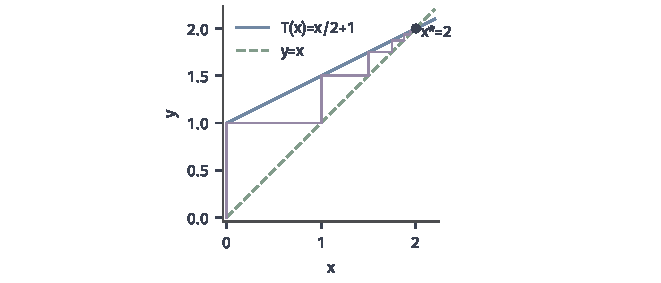
\includegraphics[width=112mm]{figures/01-mathematical-preliminaries-upper/01-mathematical-language-combinatorics-analysis-optimization/matplotlib/comprehension-additions/contraction-cobweb.pdf}
  \caption{$T(x)=x/2+1$在$[0,2]$上的七步迭代，初值$x^{(0)}=0$。蓝线是$T$，绿虚线是恒等函数，紫折线交替完成求值与复制；交点为$x^\star=2$。精确迭代为$x^{(n)}=2-2^{1-n}$，图中几何收缩对应压缩因子$1/2$。}
  \label{fig:vol1-add-contraction-cobweb}
\end{figure}

\subsubsection{带扰动的压缩迭代}

\paragraph{误差的递推估计}

若每一步只近似计算$T$，新加入的误差也会影响后续项。
设$T$满足压缩条件，精确轨迹为
$x^{(t+1)}=T(x^{(t)})$，计算轨迹为$z^{(t)}$，且每次更新满足
$d(z^{(t+1)},T(z^{(t)}))\leq\delta_t$，其中$\delta_t\geq0$。
令$e^{(t)}=d(z^{(t)},x^{(t)})$，三角不等式给出
\begin{equation}
 \begin{aligned}
 e^{(t+1)}
 &\leq d(z^{(t+1)},T(z^{(t)}))
       +d(T(z^{(t)}),T(x^{(t)}))\\
 &\leq\delta_t+\rho e^{(t)},\qquad 0\leq\rho<1.
 \end{aligned}
\label{eq:analysis-perturbed-distance-recursion}
% 保留内容迁移前的语义标签，指向同一公式。
\begingroup
\makeatletter
\let\label\ltx@label
\label{eq:prelim-perturbed-recurrence}
\endgroup
\end{equation}
这里$\rho$就是所用压缩因子。对到不动点的误差$d(z^{(t)},x^\star)$也有同一递推。
把不等式逐次代入，或对$t$归纳，得到
\begin{equation}
 e^{(t)}
 \leq \rho^t e^{(0)}
       +\sum_{s=0}^{t-1}\rho^{t-1-s}\delta_s.
\label{eq:analysis-perturbed-distance-unrolling}
% 保留内容迁移前的语义标签，指向同一公式。
\begingroup
\makeatletter
\let\label\ltx@label
\label{eq:prelim-unrolled-recurrence}
\endgroup
\end{equation}
有限展开把初始误差和各轮新增误差分开，接下来据此判断它随$t$增加的行为。
例如$t=1$时展开就是原递推；若第$t$步成立，再乘$\rho\geq0$并加$\delta_t$，
便得到第$t+1$步的展开。这样逐步验证了任意正整数步的公式。
若$\delta_s\leq\bar\delta$，则
$e^{(t)}\leq\rho^t e^{(0)}+\bar\delta(1-\rho^t)/(1-\rho)$，
所以$\limsup_t e^{(t)}\leq\bar\delta/(1-\rho)$。
这是最坏误差范围，不是断言每条计算轨迹都收敛到这个上界。

\paragraph{持续扰动与衰减扰动}

展开式中的旧误差会衰减，每轮新增误差则继续进入累计。固定初值与压缩系数，只改变新增误差是否趋零，就能看清两种误差来源。
\begin{example}[持续扰动与衰减扰动]
\label{ex:prelim-recurring-perturbations}
取$e^{(0)}=1$、$\rho=1/2$，并暂把递推中的不等号取为等号。若每步都加入
$\delta_t=0.1$，展开式给出
\[
 e^{(t)}=2^{-t}+0.1\sum_{s=0}^{t-1}2^{-s}
        =0.2+0.8\,2^{-t}.
\]
初始误差逐步消失，持续加入的误差却留下$0.2$的极限。若改为
$\delta_t=0.1/(t+1)$，扰动本身也衰减，稳定递推便使$e^{(t)}\to0$。
例如第$1$步两者都是$0.6$，第$2$步分别为$0.4$和$0.35$；差别来自第二步加入的
新误差，而不是初值不同。这里的$1/(t+1)$扰动并不可求和，几何权重仍能使其累计影响趋于零；可求和性是更强的条件。
\end{example}

\begin{figure}[htbp]
  \centering
  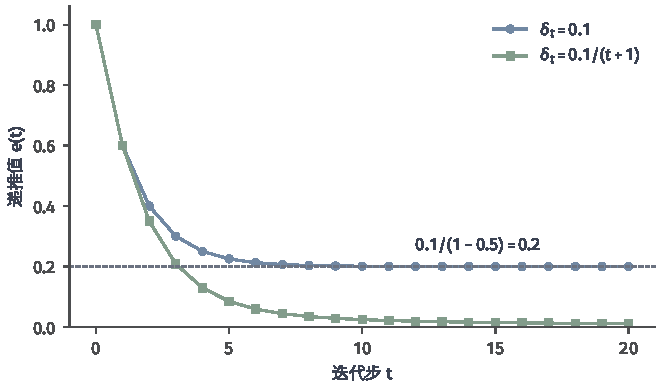
\includegraphics[width=112.0mm]{figures/01-mathematical-preliminaries-upper/01-mathematical-language-combinatorics-analysis-optimization/matplotlib/prelim-perturbed-recurrence/figure.pdf}
  \caption{相同初值与收缩系数下的两种递推。蓝线使用持续扰动，绿线使用衰减扰动；每个点都是整数步上的精确递推值，图中$e(t)$对应正文的$e^{(t)}$，灰虚线是持续扰动留下的极限$0.2$。图为教学构造。}
 \label{fig:prelim-perturbed-recurrence}
\end{figure}

衰减扰动的结论可以直接由有限展开式~\eqref{eq:analysis-perturbed-distance-unrolling}核对。
给定$\varepsilon>0$，先选$S$使$s\geq S$时$\delta_s\leq\varepsilon(1-\rho)/2$。
对$t>S$把累计和拆成两段：前$S$项是有限个旧扰动，其权重随$t$几何趋零；后面的项满足
\[
 \sum_{s=S}^{t-1}\rho^{t-1-s}\delta_s
 \leq\frac{\varepsilon(1-\rho)}2\sum_{j=0}^{t-1-S}\rho^j
 \leq\frac\varepsilon2.
\]
旧扰动项和初始误差在充分大的$t$后也不超过$\varepsilon/2$，因此总误差趋于零。
这里需要$0\leq\rho<1$、$\delta_s\to0$和有限的初始误差；只写“每步误差很小”仍不足够。

